% Options for packages loaded elsewhere
\PassOptionsToPackage{unicode}{hyperref}
\PassOptionsToPackage{hyphens}{url}
\PassOptionsToPackage{dvipsnames,svgnames,x11names}{xcolor}
%
\documentclass[
  ignorenonframetext,
  aspectratio=169,
  c]{beamer}
\usepackage{pgfpages}
\setbeamertemplate{caption}[numbered]
\setbeamertemplate{caption label separator}{: }
\setbeamercolor{caption name}{fg=normal text.fg}
\beamertemplatenavigationsymbolshorizontal
% Prevent slide breaks in the middle of a paragraph
\widowpenalties 1 10000
\raggedbottom
\setbeamertemplate{part page}{
  \centering
  \begin{beamercolorbox}[sep=16pt,center]{part title}
    \usebeamerfont{part title}\insertpart\par
  \end{beamercolorbox}
}
\setbeamertemplate{section page}{
  \centering
  \begin{beamercolorbox}[sep=12pt,center]{part title}
    \usebeamerfont{section title}\insertsection\par
  \end{beamercolorbox}
}
\setbeamertemplate{subsection page}{
  \centering
  \begin{beamercolorbox}[sep=8pt,center]{part title}
    \usebeamerfont{subsection title}\insertsubsection\par
  \end{beamercolorbox}
}
\AtBeginPart{
  \frame{\partpage}
}
\AtBeginSection{
  \ifbibliography
  \else
    \frame{\sectionpage}
  \fi
}
\AtBeginSubsection{
  \frame{\subsectionpage}
}

\usepackage{amsmath,amssymb}
\usepackage{iftex}
\ifPDFTeX
  \usepackage[T1]{fontenc}
  \usepackage[utf8]{inputenc}
  \usepackage{textcomp} % provide euro and other symbols
\else % if luatex or xetex
  \usepackage{unicode-math}
  \defaultfontfeatures{Scale=MatchLowercase}
  \defaultfontfeatures[\rmfamily]{Ligatures=TeX,Scale=1}
\fi
\usepackage{lmodern}
\usetheme[]{Luebeck}
\usecolortheme{beaver}
\ifPDFTeX\else  
    % xetex/luatex font selection
\fi
% Use upquote if available, for straight quotes in verbatim environments
\IfFileExists{upquote.sty}{\usepackage{upquote}}{}
\IfFileExists{microtype.sty}{% use microtype if available
  \usepackage[]{microtype}
  \UseMicrotypeSet[protrusion]{basicmath} % disable protrusion for tt fonts
}{}
\makeatletter
\@ifundefined{KOMAClassName}{% if non-KOMA class
  \IfFileExists{parskip.sty}{%
    \usepackage{parskip}
  }{% else
    \setlength{\parindent}{0pt}
    \setlength{\parskip}{6pt plus 2pt minus 1pt}}
}{% if KOMA class
  \KOMAoptions{parskip=half}}
\makeatother
\usepackage{xcolor}
\newif\ifbibliography
\setlength{\emergencystretch}{3em} % prevent overfull lines
\setcounter{secnumdepth}{-\maxdimen} % remove section numbering


\providecommand{\tightlist}{%
  \setlength{\itemsep}{0pt}\setlength{\parskip}{0pt}}\usepackage{longtable,booktabs,array}
\usepackage{calc} % for calculating minipage widths
\usepackage{caption}
% Make caption package work with longtable
\makeatletter
\def\fnum@table{\tablename~\thetable}
\makeatother
\usepackage{graphicx}
\makeatletter
\def\maxwidth{\ifdim\Gin@nat@width>\linewidth\linewidth\else\Gin@nat@width\fi}
\def\maxheight{\ifdim\Gin@nat@height>\textheight\textheight\else\Gin@nat@height\fi}
\makeatother
% Scale images if necessary, so that they will not overflow the page
% margins by default, and it is still possible to overwrite the defaults
% using explicit options in \includegraphics[width, height, ...]{}
\setkeys{Gin}{width=\maxwidth,height=\maxheight,keepaspectratio}
% Set default figure placement to htbp
\makeatletter
\def\fps@figure{htbp}
\makeatother

\makeatletter
\@ifpackageloaded{tcolorbox}{}{\usepackage[skins,breakable]{tcolorbox}}
\@ifpackageloaded{fontawesome5}{}{\usepackage{fontawesome5}}
\definecolor{quarto-callout-color}{HTML}{909090}
\definecolor{quarto-callout-note-color}{HTML}{0758E5}
\definecolor{quarto-callout-important-color}{HTML}{CC1914}
\definecolor{quarto-callout-warning-color}{HTML}{EB9113}
\definecolor{quarto-callout-tip-color}{HTML}{00A047}
\definecolor{quarto-callout-caution-color}{HTML}{FC5300}
\definecolor{quarto-callout-color-frame}{HTML}{acacac}
\definecolor{quarto-callout-note-color-frame}{HTML}{4582ec}
\definecolor{quarto-callout-important-color-frame}{HTML}{d9534f}
\definecolor{quarto-callout-warning-color-frame}{HTML}{f0ad4e}
\definecolor{quarto-callout-tip-color-frame}{HTML}{02b875}
\definecolor{quarto-callout-caution-color-frame}{HTML}{fd7e14}
\makeatother
\makeatletter
\@ifpackageloaded{caption}{}{\usepackage{caption}}
\AtBeginDocument{%
\ifdefined\contentsname
  \renewcommand*\contentsname{Table of contents}
\else
  \newcommand\contentsname{Table of contents}
\fi
\ifdefined\listfigurename
  \renewcommand*\listfigurename{List of Figures}
\else
  \newcommand\listfigurename{List of Figures}
\fi
\ifdefined\listtablename
  \renewcommand*\listtablename{List of Tables}
\else
  \newcommand\listtablename{List of Tables}
\fi
\ifdefined\figurename
  \renewcommand*\figurename{Figure}
\else
  \newcommand\figurename{Figure}
\fi
\ifdefined\tablename
  \renewcommand*\tablename{Table}
\else
  \newcommand\tablename{Table}
\fi
}
\@ifpackageloaded{float}{}{\usepackage{float}}
\floatstyle{ruled}
\@ifundefined{c@chapter}{\newfloat{codelisting}{h}{lop}}{\newfloat{codelisting}{h}{lop}[chapter]}
\floatname{codelisting}{Listing}
\newcommand*\listoflistings{\listof{codelisting}{List of Listings}}
\makeatother
\makeatletter
\makeatother
\makeatletter
\@ifpackageloaded{caption}{}{\usepackage{caption}}
\@ifpackageloaded{subcaption}{}{\usepackage{subcaption}}
\makeatother
\ifLuaTeX
  \usepackage{selnolig}  % disable illegal ligatures
\fi
\usepackage{bookmark}

\IfFileExists{xurl.sty}{\usepackage{xurl}}{} % add URL line breaks if available
\urlstyle{same} % disable monospaced font for URLs
\hypersetup{
  pdftitle={Conception et Innovation -- CI3},
  pdfauthor={MdC. Fabio Cruz; MdC Alaa Hassan},
  colorlinks=true,
  linkcolor={Blue},
  filecolor={Maroon},
  citecolor={Blue},
  urlcolor={Blue},
  pdfcreator={LaTeX via pandoc}}

\title{Conception et Innovation -- CI3}
\subtitle{Schema Cinématique}
\author{MdC. Fabio Cruz \and MdC Alaa Hassan}
\date{2023-03-20}
\institute{Université de Lorraine \textbar{} ENSGSI}

\begin{document}
\frame{\titlepage}

\renewcommand*\contentsname{Organisation de la presentation}
\begin{frame}[allowframebreaks]
  \frametitle{Organisation de la presentation}
  \tableofcontents[hideallsubsections]
\end{frame}
\section{Modélisation des liaisons
mécaniques}\label{moduxe9lisation-des-liaisons-muxe9caniques}

\subsection{Définition}\label{duxe9finition}

\begin{frame}{Définition}
\textbf{Mécanisme}:

On appelle mécanisme, un \emph{ensemble de pièces mécaniques} reliées
entre elles par des \emph{liaisons}, en vue de réaliser une fonction
déterminée.

\begin{figure}

\begin{minipage}{0.70\linewidth}
Nous admettrons que les pièces mécaniques peuvent être modélisées par
des \textbf{solides indéformables}.\end{minipage}%
%
\begin{minipage}{0.30\linewidth}

\includegraphics[width=0.9\textwidth,height=\textheight]{CM3/turbina.gif}

\subcaption{\label{}Exemple de mécanisme : un micromoteur de modélisme}
\end{minipage}%

\end{figure}%
\end{frame}

\subsection{Solides Indeformables}\label{solides-indeformables}

\begin{frame}{Solides Indeformables}
Le solide possède une \emph{masse constante} et un \emph{volume} dont
les \textbf{limites sont invariantes} quelles que soient les actions
extérieures auxquelles il est soumis.

\begin{figure}

\begin{minipage}{0.70\linewidth}

\begin{tcolorbox}[enhanced jigsaw, colback=white, left=2mm, toprule=.15mm, arc=.35mm, bottomtitle=1mm, breakable, colframe=quarto-callout-note-color-frame, title=\textcolor{quarto-callout-note-color}{\faInfo}\hspace{0.5em}{Conséquence géométrique}, opacitybacktitle=0.6, bottomrule=.15mm, toptitle=1mm, titlerule=0mm, coltitle=black, colbacktitle=quarto-callout-note-color!10!white, leftrule=.75mm, opacityback=0, rightrule=.15mm]

La distance entre deux points quelconques d'un solide indéformable est
invariable dans un \textbf{Repère donneé}

\end{tcolorbox}

\end{minipage}%
%
\begin{minipage}{0.30\linewidth}

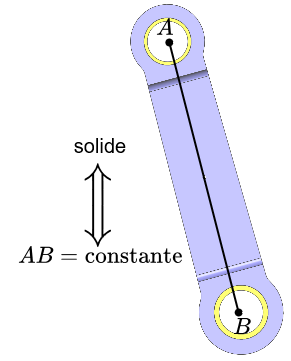
\includegraphics[width=0.9\textwidth,height=\textheight]{CM3/Solide-indeformable.png}

\subcaption{\label{}Exemple de mécanisme : un micromoteur de modélisme}
\end{minipage}%

\end{figure}%
\end{frame}

\subsection{Repère}\label{repuxe8re}

\begin{frame}{Repère}
Pour connaitre la position de tous ses points dans l'espace, il suffit
de connaitre la position d'un repère lié à ce solide.

\begin{figure}

\begin{minipage}{0.60\linewidth}
\textbf{Repère de référence}: \(R(O, \vec{x}, \vec{y}, \vec{z})\)
\textbf{Repère de lié au solide.}:
\(R(O_1, \vec{x_1}, \vec{y_1}, \vec{z_1})\)\end{minipage}%
%
\begin{minipage}{0.40\linewidth}
\begin{center}
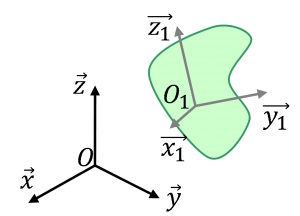
\includegraphics[width=0.9\textwidth,height=\textheight]{CM3/Repere.png}
\end{center}
\end{minipage}%

\end{figure}%

\pause

La position du solide dans l'espace, est déterminée par \emph{6
paramètres indépendants}

\begin{enumerate}
\tightlist
\item
  Position du point \(O_1\) → \textbf{3 Coordonnées}
\item
  Orientation de \(\vec{x_1}, \vec{y_1}, \vec{z_1})\) par rapport à
  \(R(O, \vec{x}, \vec{y}, \vec{z})\) → \textbf{3 Angles}
\end{enumerate}
\end{frame}

\begin{frame}{Repère}
\phantomsection\label{repuxe8re-1}
Exemple : repère local lié au solide 2 (la bielle) et repère de
référence, lié au solide 0 (le bâti)

\begin{figure}

\begin{minipage}{0.50\linewidth}
\begin{center}
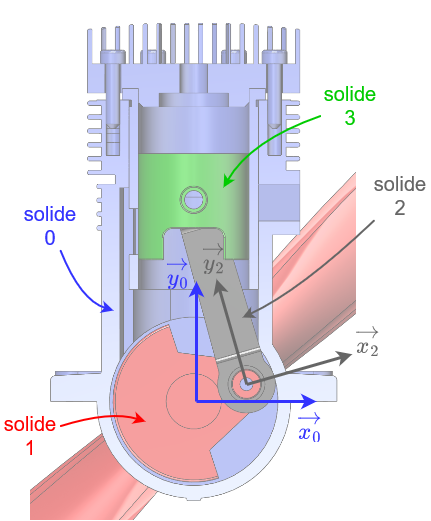
\includegraphics[width=0.9\textwidth,height=\textheight]{CM3/Repere-01.png}
\end{center}
\end{minipage}%
%
\begin{minipage}{0.50\linewidth}
\begin{center}
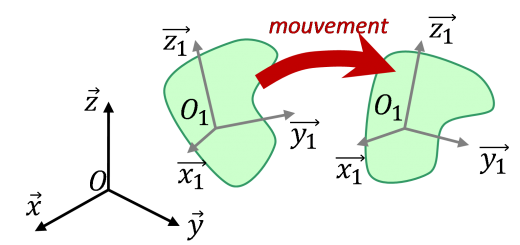
\includegraphics[width=0.9\textwidth,height=\textheight]{CM3/Repere-02.gif}
\end{center}
\end{minipage}%

\end{figure}%
\end{frame}

\begin{frame}{Repère}
\phantomsection\label{repuxe8re-2}
Example 2
\end{frame}

\subsection{Degree de liberté}\label{degree-de-libertuxe9}

\begin{frame}{Degree de liberté}
Il existe deux mouvements élémentaires entre les solides :

\begin{enumerate}
\tightlist
\item
  Le mouvement de \textbf{TRANSLATION (RECTILIGNE)} : les trajectoires
  de tous les points du solide sont des droites parallèles.
\item
  Le mouvement de \textbf{ROTATION} : les trajectoires de chaque point
  sont des cercles coaxiaux.
\end{enumerate}

\begin{figure}

\begin{minipage}{0.70\linewidth}
On appelle \emph{libertés} d'un solide par rapport à un référentiel, les
mouvements indépendants de ce solide pour passer d'une position à une
autre.\end{minipage}%
%
\begin{minipage}{0.30\linewidth}
\begin{center}
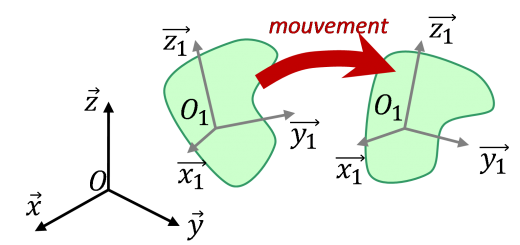
\includegraphics[width=1\textwidth,height=\textheight]{CM3/Repere-02.png}
\end{center}
\end{minipage}%

\end{figure}%
\end{frame}

\begin{frame}{Degree de Liberte}
\phantomsection\label{degree-de-liberte}
Il existe deux mouvements élémentaires entre les solides :

\begin{enumerate}
\tightlist
\item
  Le mouvement de \textbf{TRANSLATION (RECTILIGNE)} : les trajectoires
  de tous les points du solide sont des droites parallèles.

  \begin{itemize}
  \tightlist
  \item
    \(T_x, T_y, T_z\) selon \((x,y,z)\)
  \end{itemize}
\item
  Le mouvement de \textbf{ROTATION} : les trajectoires de chaque point
  sont des cercles coaxiaux.

  \begin{itemize}
  \tightlist
  \item
    \(R_x, R_y, R_z\) autour des axes \((x,y,z)\)
  \end{itemize}
\end{enumerate}

\begin{figure}

\begin{minipage}{0.70\linewidth}
\textbf{6 Degrees de liberté}\end{minipage}%
%
\begin{minipage}{0.30\linewidth}
\begin{center}
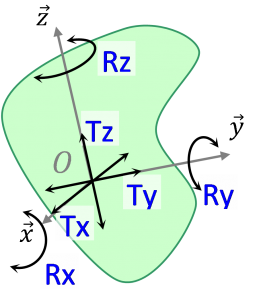
\includegraphics[width=0.9\textwidth,height=\textheight]{CM3/Degrees-liberte.pdf}
\end{center}
\end{minipage}%

\end{figure}%
\end{frame}

\subsection{Notion de liaison}\label{notion-de-liaison}

\begin{frame}{Notion de liaison}
On appelle \textbf{liaison} entre deux solides l'ensemble des couples de
surfaces en contact entre ces deux solides, \textbf{visant à diminuer la
mobilité entre ces deux solides}.

\textbf{Zones de Contacts}

\begin{figure}[H]

{\centering 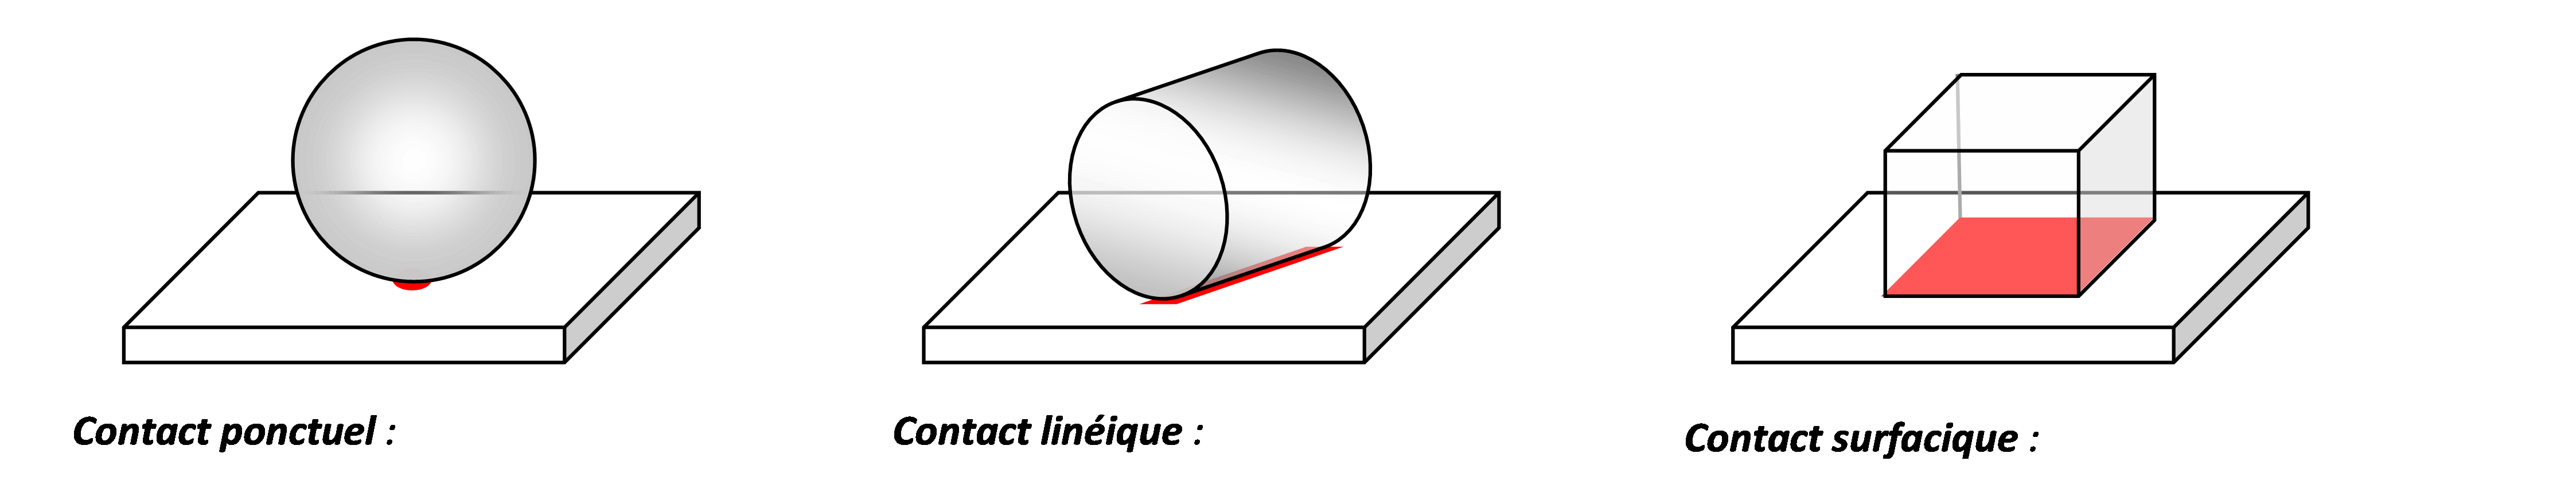
\includegraphics[width=0.8\textwidth,height=\textheight]{CM3/Contact.png}

}

\caption{Contact}

\end{figure}%
\end{frame}

\subsection{Degrés de liberté/de liaison d'une
liaison}\label{degruxe9s-de-libertuxe9de-liaison-dune-liaison}

\begin{frame}{Degrés de liberté/de liaison d'une liaison}
Les \emph{degrés de liberté d'une liaison} sont \textbf{les déplacements
élémentaires indépendants} autorisés par cette liaison.
\end{frame}

\subsection{Les Liaisons Mécaniques
Elementaires}\label{les-liaisons-muxe9caniques-elementaires}

\begin{frame}{Encastrement}
\phantomsection\label{encastrement}
\begin{center}
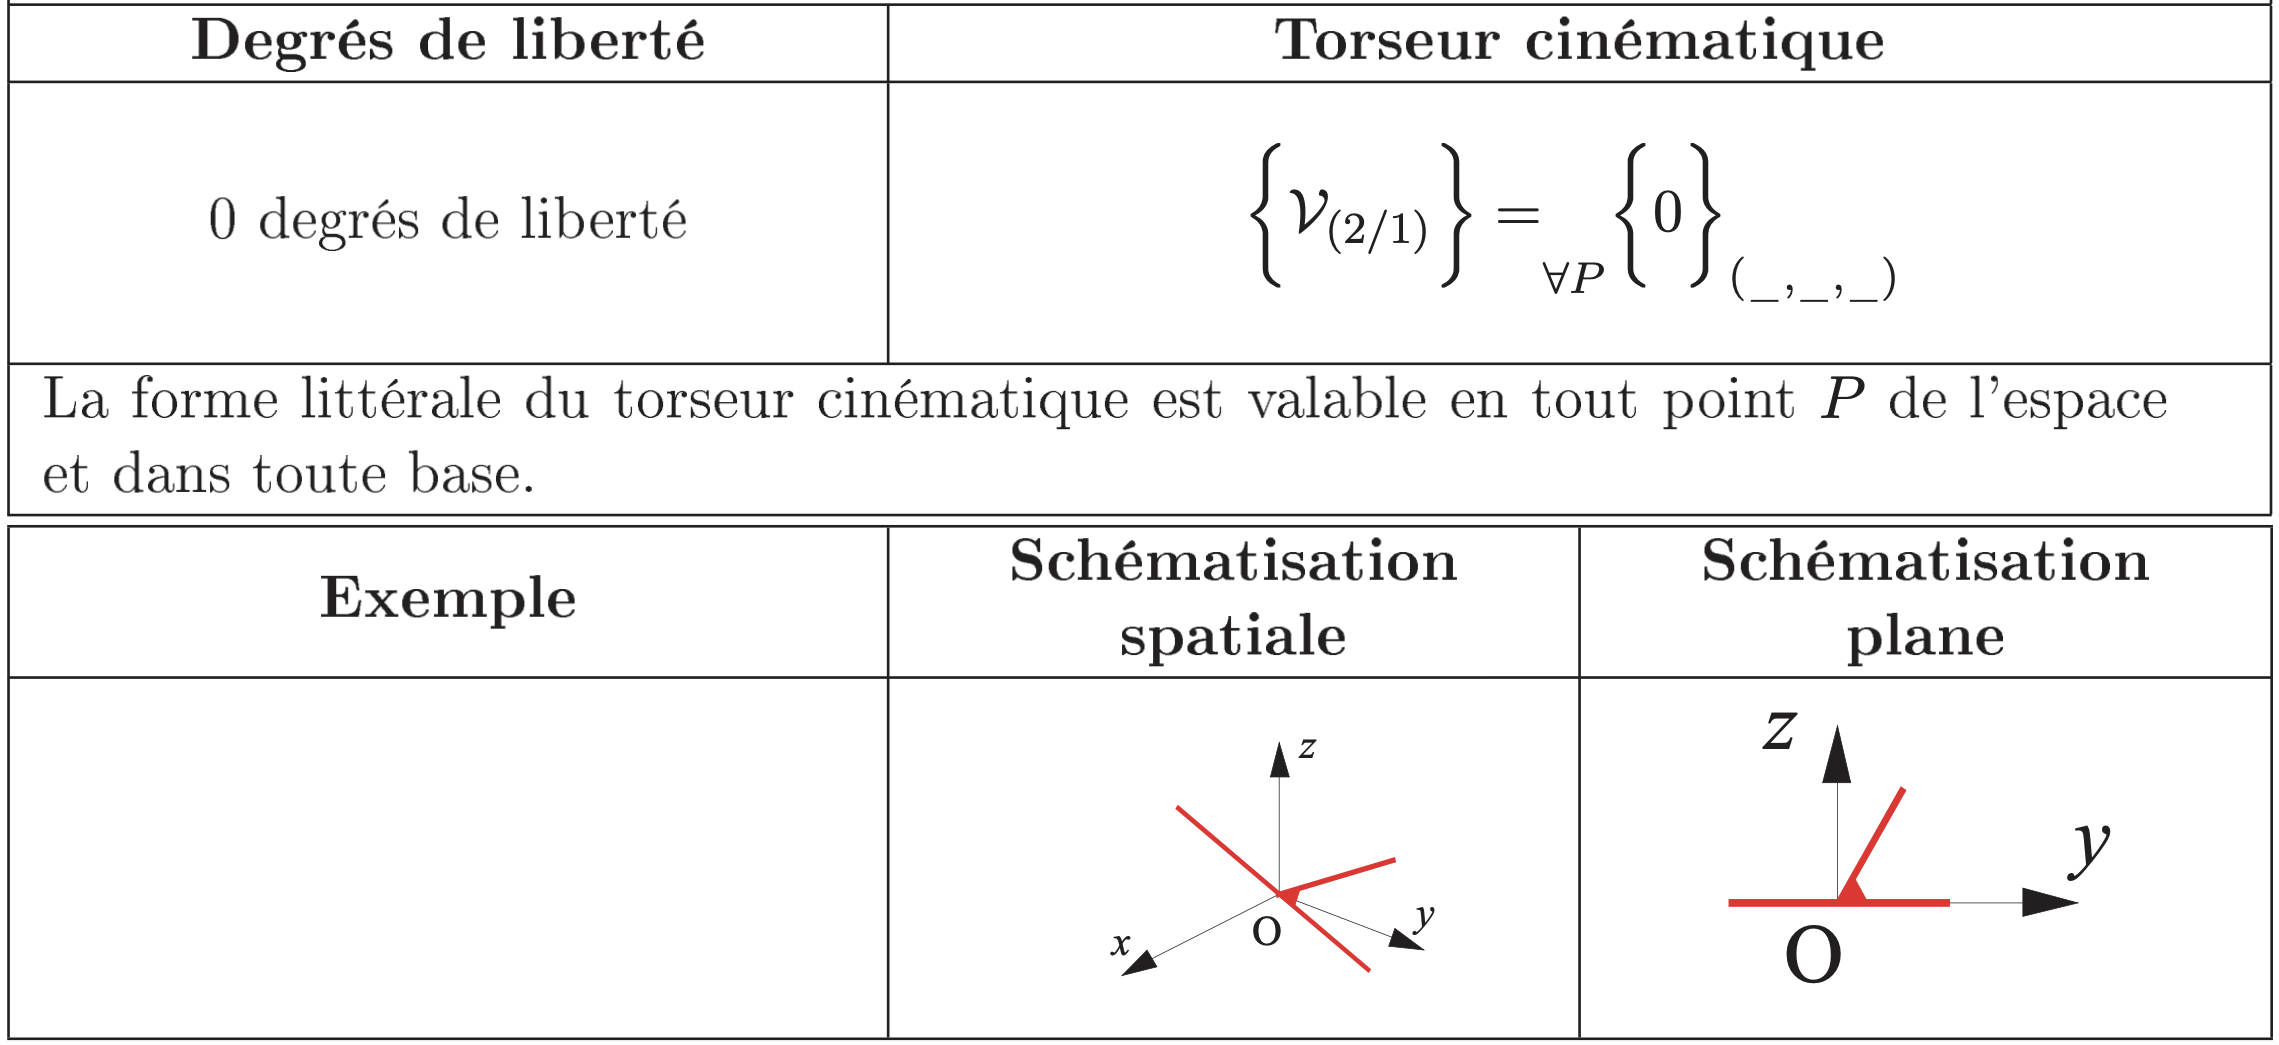
\includegraphics[width=0.8\textwidth,height=\textheight]{CM3/Encastrement.png}
\end{center}
\end{frame}

\subsection{Les Liaisons Mécaniques
Elementaires}\label{les-liaisons-muxe9caniques-elementaires-1}

\begin{frame}{Les Liaisons Mécaniques Elementaires}
\begin{longtable}[]{@{}
  >{\raggedright\arraybackslash}p{(\columnwidth - 6\tabcolsep) * \real{0.2623}}
  >{\raggedright\arraybackslash}p{(\columnwidth - 6\tabcolsep) * \real{0.2623}}
  >{\raggedright\arraybackslash}p{(\columnwidth - 6\tabcolsep) * \real{0.1803}}
  >{\raggedright\arraybackslash}p{(\columnwidth - 6\tabcolsep) * \real{0.2951}}@{}}
\toprule\noalign{}
\begin{minipage}[b]{\linewidth}\raggedright
\textbf{Liaison}
\end{minipage} & \begin{minipage}[b]{\linewidth}\raggedright
\textbf{Symbole}
\end{minipage} & \begin{minipage}[b]{\linewidth}\raggedright
\textbf{Degree de Liberté}
\end{minipage} & \begin{minipage}[b]{\linewidth}\raggedright
\textbf{Torseur cinématique}
\end{minipage} \\
\midrule\noalign{}
\endhead
Encastrement \begin{center}
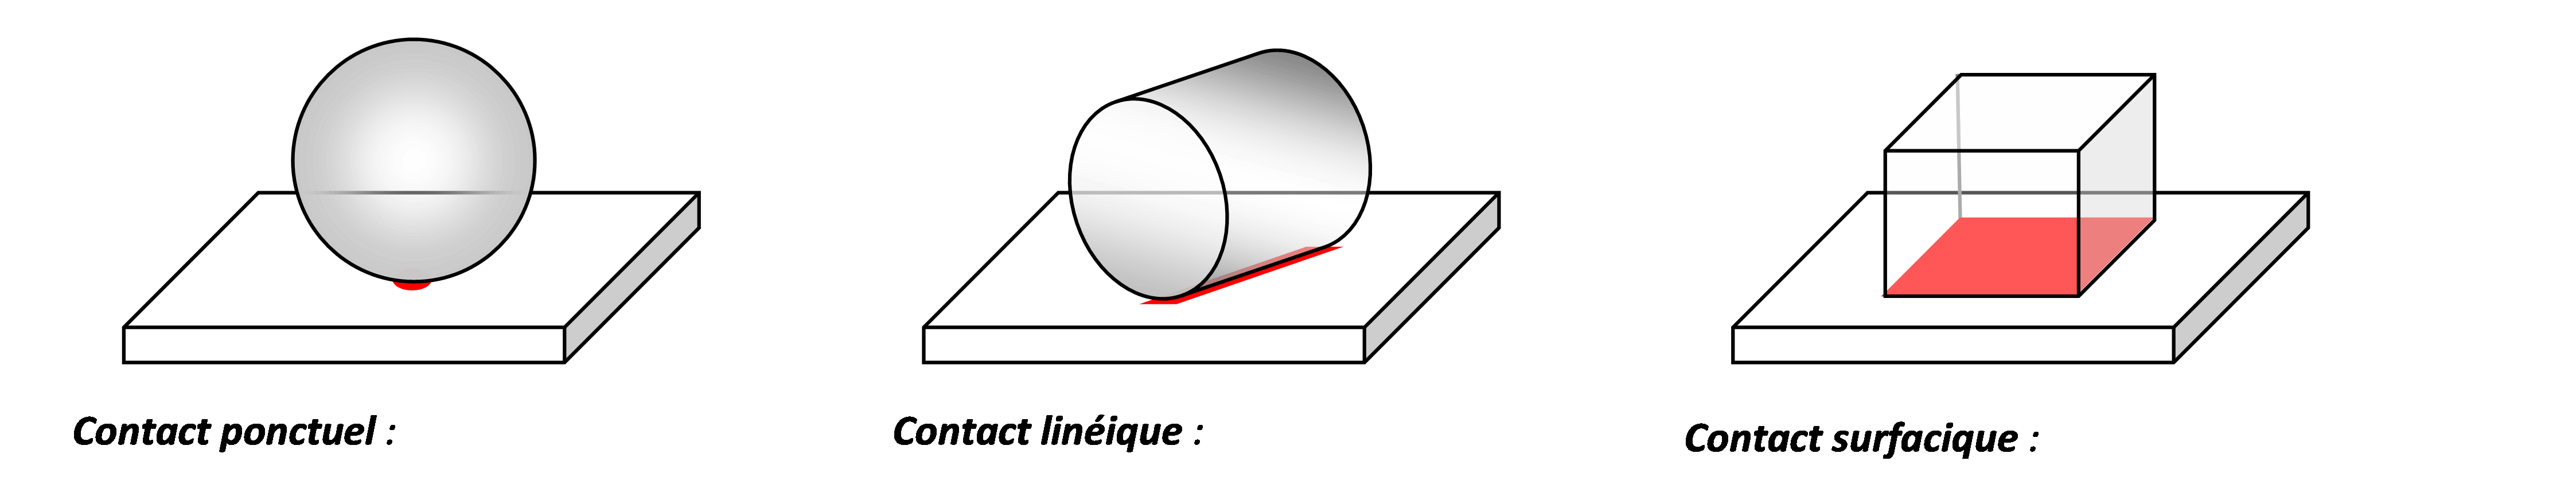
\includegraphics[width=0.8\textwidth,height=\textheight]{CM3/Contact.png}
\end{center}
& 2.05 & 2.05 & 2.05 \\
\bottomrule\noalign{}
\end{longtable}
\end{frame}

\section{Élaboration d'un schéma
cinématique}\label{uxe9laboration-dun-schuxe9ma-cinuxe9matique}

\subsection{Définition}\label{duxe9finition-1}

\begin{frame}{Définition}
Le schéma cinématique d'un mécanisme est un **modèle filaire du
mécanisme utilisant les symboles normalisés des liaisons.

Ce modèle est utile tant au niveau de la conception que de l'analyse à
posteriori pour réaliser l'étude cinématique ou dynamique (trajectoire,
vitesse, efforts, etc.)
\end{frame}

\section{Exemple}\label{exemple}



\end{document}
